% -------- Figures & Tables Reference -------%

Figures are referred to as e.g. Fig.~\ref{}, and tables as e.g. Table~\ref{tab:example_table}.

% Example figure
\begin{figure}
	% Allowable file formats are eps or ps if compiling using latex or pdf, png, jpg if compiling using pdflatex
	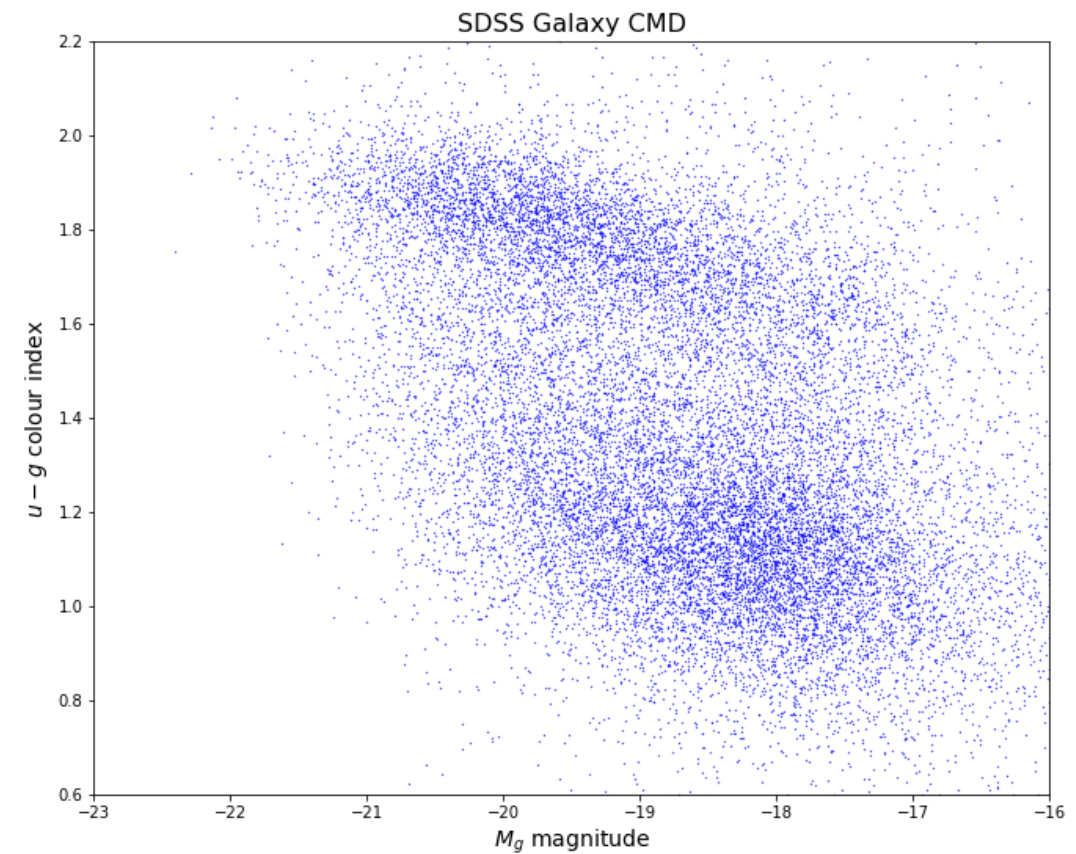
\includegraphics[width=\columnwidth]{images/galaxyCMD.PNG}
    \caption{Galaxy colour-magnitude diagram: $u-g$ colour index versus $M_g$ magnitude. The bimodality of the distribution is discussed in the text.}
    \label{fig:CMD1}
\end{figure}

% Example table
\begin{table}
	\centering
	\caption{This is an example table. Captions appear above each table.
	Remember to define the quantities, symbols and units used.}
	\label{tab:example_table}
	\begin{tabular}{lccr} % four columns, alignment for each
		\hline
		A & B & C & D\\
		\hline
		1 & 2 & 3 & 4\\
		2 & 4 & 6 & 8\\
		3 & 5 & 7 & 9\\
		\hline
	\end{tabular}
\end{table}

\subsection{Special symbols}


\begin{table}
 \caption{Additional commands for special symbols commonly used in astronomy. These can be used anywhere.}
 \label{tab:anysymbols}
 \begin{tabular}{lll}
  \hline
  Command & Output & Meaning\\
  \hline
  \verb'\sun' & \sun & Sun, solar\\[2pt] % additional height spacing for enhanced symbol legibility
  \verb'\earth' & \earth & Earth, terrestrial\\[2pt]
  \verb'\micron' & \micron & microns\\[2pt]
  \verb'\degr' & \degr & degrees\\[2pt]
  \verb'\arcmin' & \arcmin & arcminutes\\[2pt]
  \verb'\arcsec' & \arcsec & arcseconds\\[2pt]
  \verb'\fdg' & \fdg & fraction of a degree\\[2pt]
  \verb'\farcm' & \farcm & fraction of an arcminute\\[2pt]
  \verb'\farcs' & \farcs & fraction of an arcsecond\\[2pt]
  \verb'\fd' & \fd & fraction of a day\\[2pt]
  \verb'\fh' & \fh & fraction of an hour\\[2pt]
  \verb'\fm' & \fm & fraction of a minute\\[2pt]
  \verb'\fs' & \fs & fraction of a second\\[2pt]
  \verb'\fp' & \fp & fraction of a period\\[2pt]
  \verb'\diameter' & \diameter & diameter\\[2pt]
  \verb'\sq' & \sq & square, Q.E.D.\\[2pt]
  \hline
 \end{tabular}
\end{table}

\begin{table}
 \caption{Additional commands for mathematical symbols. These can only be used in maths mode.}
 \label{tab:mathssymbols}
 \begin{tabular}{lll}
  \hline
  Command & Output & Meaning\\
  \hline
  \verb'\upi' & $\upi$ & upright pi\\[2pt] % additional height spacing for enhanced symbol legibility
  \verb'\umu' & $\umu$ & upright mu\\[2pt]
  \verb'\upartial' & $\upartial$ & upright partial derivative\\[2pt]
  \verb'\lid' & $\lid$ & less than or equal to\\[2pt]
  \verb'\gid' & $\gid$ & greater than or equal to\\[2pt]
  \verb'\la' & $\la$ & less than of order\\[2pt]
  \verb'\ga' & $\ga$ & greater than of order\\[2pt]
  \verb'\loa' & $\loa$ & less than approximately\\[2pt]
  \verb'\goa' & $\goa$ & greater than approximately\\[2pt]
  \verb'\cor' & $\cor$ & corresponds to\\[2pt]
  \verb'\sol' & $\sol$ & similar to or less than\\[2pt]
  \verb'\sog' & $\sog$ & similar to or greater than\\[2pt]
  \verb'\lse' & $\lse$ & less than or homotopic to \\[2pt]
  \verb'\gse' & $\gse$ & greater than or homotopic to\\[2pt]
  \verb'\getsto' & $\getsto$ & from over to\\[2pt]
  \verb'\grole' & $\grole$ & greater over less\\[2pt]
  \verb'\leogr' & $\leogr$ & less over greater\\
  \hline
 \end{tabular}
\end{table}
